
\chapter{Week1}

\section{Tuesday}\index{Tuesday_lecture}

\subsection{Introduction}
\subsubsection{\textit{Why do you learn Linear Algebra?}}
\paragraph{Important: LA + Calculus + Probability}

Every SSE student should learn {\emph{Linear Algebra}}, {\emph{Calculus}}, and {\emph{Probability}} to build strong fundation.

\paragraph{Practical: Computation}

Linear Algebra is more widely used than Calculus since we could use this {\emph{powerful}} tool to do discrete computation. (As we know, we can use calculus to deal with something continuous. But how do we do integration when facing lots of \emph{discrete data}? But linear algebra can help us deal with these data.)

\paragraph{Visualize} 

Conncect between \emph{Geometry} and \emph{Algebra}.

Let's take an easy example:
\begin{example}

Let $v$ and $w$ donate two vectors as below:
\[
\begin{array}{ll}
v= \begin{bmatrix}
1 \\ 2
\end{bmatrix},
&
w = \begin{bmatrix}
3 \\ 4
\end{bmatrix}.
\end{array}
\]

Then we can donate these two vectors in the graph:
\begin{center}
\setlength{\unitlength}{0.5 cm}
\begin{picture}(15,3)\thicklines
\put(0,0){\vector(1,2){1}} \put(0,0){\vector(1,0){2}}
\put(-0.2,1){$v$} \put(1,-0.6){$w$} \put(3.2,2){$v+w$}
\put(1,2){\line(1,0){0.2}} \put(0,0){\vector(3,2){3}}
\put(1.4,2){\line(1,0){0.2}} \put(1.8,2){\line(1,0){0.2}}
\put(2.2,2){\line(1,0){0.2}} \put(2.6,2){\line(1,0){0.2}}
\put(8,1){\vector(1,1){2}} \put(8,1){\vector(2,-1){2}}
\put(10,0){\vector(0,1){3}} \put(8.3,1.9){$v$} \put(8.3,0){$w$}
\put(10.5,1){$v-w$}
\end{picture}
\end{center}

And we can also add two vectors to get $v+w$. Additionally, we can change the coefficients in front of $v$ and $w$ to get $v-w$.

In two dimension space, we can visualize the vector in the coordinate. Then let's watch the \emph{three} dimension space.There are four vectors $u$,$v$,$w$ and $b$. We can also denote it in coordinate.

Here we raise a question: Can we denote vector $b$ as a linear combination with the three vectors $u$, $v$, and $w$? That is to say,
\begin{quotation}
Is there exists coefficients $x_1$, $x_2$, $x_3$ such that 
\[
x_1 \begin{pmatrix}
1 \\ 1 \\ 1
\end{pmatrix}+
x_2 \begin{pmatrix}
1 \\ 2 \\ 3
\end{pmatrix}+
x_3 \begin{pmatrix}
1 \\ 3 \\ 4
\end{pmatrix}=
\begin{pmatrix}
2 \\ 5 \\ 7
\end{pmatrix}?
\]
\end{quotation}

Then we only need to solve the system of equations 
\[\left\{ \begin{gathered}
x_1 + x_2 + x_3 = 2 \\
x_1 + 2x_2 + 3x_3 = 5 \\
x_1 + 3x_2 + 4x_3 = 7
\end{gathered} \right.
\implies \begin{pmatrix}
x_1 \\ x_2 \\ x_3
\end{pmatrix} = \begin{pmatrix}
0 \\ 1 \\ 1
\end{pmatrix}
\]
\end{example}
\paragraph{Abstract: Broad Applications}

Don't worry, broad doesn't mean boring. Instead, it means Linear Algebra can applied to lots of applications.

For example, if we denote a sequence of infinite numbers as a tuple that contains infinite numbers, and we denote this tuple as a vector, then we could build \emph{an infinite banach space.} Moreover, Given a function $f:\mathbb{R} \to \mathbb{R}$, we can describle a set of functions as a tuple, then we could build a \emph{function space}. These abstract knowledge may be not covered in this course. We will learn it in future courses.

\subsubsection{What is Linear Algebra?}
The central problem in math is to \emph{solve equations}. And equations can be seperated into two parts, \emph{nonlinear} and \emph{linear} ones. 

Let's look an example of Nonlinear equations below:
\[ 
\left\{ \begin{gathered}
3x_1x_2 + 5x_1^2 + 6x_2 = 9 \\
x_1x_2^2 + 5x_1 + 7x_2^2 = 10
\end{gathered}
\right.
\]

Well, it is a little bit complicated. We don't find a efficient algorithm to solve these equations. But in algebraic geometry course we will solve some nonlinear equations.

What you need to know about in this course is the linear equations and the methodology to solve it.

\begin{definition}[Linear Equations]
A linear equation in $n$ unknowns is the equation of the form
\[
a_1x_1 + a_2x_2 +\dots + a_nx_n = b,
\]
where $a_1,a_2,\dots,a_n,b$ are real numbers and $x_1,x_2,\dots,x_n$ are variables
\end{definition}

\begin{definition}[Linear System of Equations]
Linear system of $m$ equations in $n$ unknowns is the system of the form

\begin{gather}
a_{11}x_1 + a_{12}x_2 + \dots + a_{1n}x_n = b_1 \notag \\ 
a_{21}x_1 + a_{22}x_2 + \dots + a_{23}x_n = b_2 \notag \\
\dots 	\notag 	\\
a_{m1}x_1 + a_{m2}x_2 + \dots + a_{m3}x_n = b_m , \label{Eq:1.1}
\end{gather}
where $a_{ij}$ and the $b_i$ are all real numbers. We refer to (\ref{Eq:1})as $m \times n$ \emph{linear systems}.
\end{definition}

 
%------------------------------------------------

\subsection{Gaussian Elimination}

Here we mainly focus on $n \times n$ system of equations. 

\begin{example}
Let's recall how to solve a $2 \times 2$ system equatons as below:
\begin{align}
1x_1 + 2x_2 &= 5\label{Eq:1.2}\\
4x_1 + 5x_2 &=14\label{Eq:1.3}.
\end{align}

We can simplify the equation system above into the form (\emph{Augmented matrix}):
\[
\left[
\begin{array}{@{}cc|c@{}}
1 & 2 & 5 \\
4 & 5 & 14
\end{array}
\right]
\]

Secondly, by adding $(-4)\times(\ref{Eq:1.2})$ into (\ref{Eq:1.3}), we obtain:
\begin{align}
{1}x_1 + 2x_2 &=5\label{Eq:1.4}\\
0x_1 + (-3)x_2 &= -6\label{Eq:1.5}
\end{align}

Thirdly, by multiplying $-(1/3)$ of (\ref{Eq:1.5}), we obtain:
\begin{align}
{1}x_1 + 2x_2 &=5 \label{Eq:1.6}\\
1x_2 &= 2\label{Eq:1.7}
\end{align}

Fourthly, by adding $(-2)\times(\ref{Eq:1.7})$ into $(\ref{Eq:1.6})$, we obtain:
\begin{align}
{1}x_1 + 0x_2 &=1 	\\
1x_2 &= 2 
\end{align}

Here we get the solution $(x_1=1, x_2=2)$, and we could write the above process with augmented matrix form:
\[
\left[
\begin{array}{@{}cc|c@{}}
1 & 2 & 5 \\
4 & 5 & 14
\end{array}
\right]
\implies
\left[
\begin{array}{@{}cc|c@{}}
1 & 2 & 5 \\
0& -3 & -6
\end{array}
\right]
\implies
\left[
\begin{array}{@{}cc|c@{}}
1 & 2 & 5 \\
0& 1 & 2
\end{array}
\right]
\implies
\left[
\begin{array}{@{}cc|c@{}}
1 & 0 & 1 \\
0& 1 & 2
\end{array}
\right].
\]
\end{example}

The method shown above is called \emph{Gaussian Elimination}. Here we give a strict definition for Augmented matrix:
\begin{definition}[Augmented matrix]
For the system of equations
\begin{gather}
a_{11}x_1 + a_{12}x_2 + \dots + a_{1n}x_n = b_1 \notag \\ 
a_{21}x_1 + a_{22}x_2 + \dots + a_{2n}x_n = b_2 \notag \\
\dots 	\notag 	\\
a_{m1}x_1 + a_{m2}x_2 + \dots + a_{mn}x_n = b_m , \label{eq:linear system equations_2}
\end{gather}
the corresponding augmented matrix is given by 
\[
\left[
\begin{array}{@{}cccc|c@{}}
a_{11} & a_{12} & \dots & a_{1n} &  b_1 \\
a_{21} & a_{22} & \dots & a_{2n} &  b_2 \\
\vdots    & \vdots    & \ddots & \vdots    & \vdots \\
a_{m1} & a_{m2} & \cdots & a_{mn} &   b_n
\end{array}
\right].
\]
\end{definition}

We give the definition for a new term \emph{pivot}:
\begin{definition}[pivot]
Returning to the example, we find after third step the matrix is given by 
\[
\left[
\begin{array}{@{}cc|c@{}}
1 & 2 & 5 \\
0 & 1 & 2
\end{array}
\right].
\]

We find that the second row will be used to eliminate the element in the second column of the first row. Here we refer to the second row as the \emph{pivot
row}. The first nonzero entry in the pivotal row is called the \emph{pivot}. For the example case, the element in the second column of the second row is the pivot.
\end{definition}

\subsubsection{How to visualize the system of equation?}
Here we try to visualize the system of equation $
\left \{	\begin{gathered}
1x_1 + 2x_2 =5	\\
4x_1 + 5x_2 = 14 
\end{gathered}	\right.$:

\paragraph{Row Picture} Focusing on the row of the system of equation, we can denote each equation as a line on the coordinate axis. And the solution denote the coordinate.

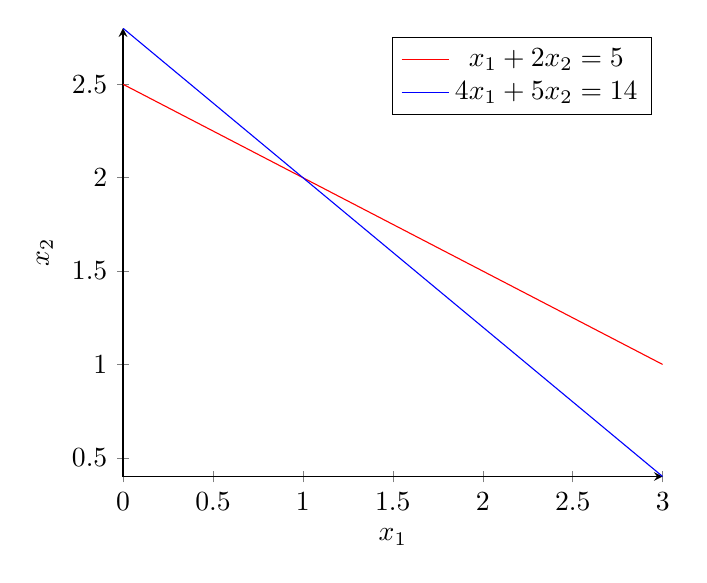
\begin{tikzpicture}
\begin{axis}[
    axis lines = left,
    xlabel = $x_1$,
    ylabel = {$x_2$},
]
%Below the red parabola is defined
\addplot [
    domain=0:3, 
    samples=100, 
    color=red,
]
{2.5-0.5*x};
\addlegendentry{$x_1+2x_2=5$}
%Here the blue parabloa is defined
\addplot [
    domain=0:3, 
    samples=100, 
    color=blue,
    ]
    {-0.8*x+2.8};
\addlegendentry{$4x_1+5x_2=14$}
\end{axis}
\end{tikzpicture}
\paragraph{Column Picture} Focusing on the column of the system of equation, we can denote 
$\begin{bmatrix}
1\\4
\end{bmatrix}$ and $\begin{bmatrix}
2\\5
\end{bmatrix}
$ as vectors in coordinate axis. {Could the linear combinations of these two vectors form the vector}
$\begin{bmatrix}
5\\14
\end{bmatrix}$?  If we denote $x_1$ and $x_2$ as coefficients, it suffices to solve the equation 
$
x_1\begin{bmatrix}
1\\4
\end{bmatrix} + x_2\begin{bmatrix}
2\\5
\end{bmatrix} = \begin{bmatrix}
5\\14
\end{bmatrix}$.

\subsubsection{The solutions of the Linear System of Equations}
The solution to linear system equation could only be \emph{unique}, \emph{infinite}, or \emph{empty}. Let's talk about it case by case in graphic way:
\paragraph{Case 1: unique solution} If two lines intersect at one point, then there is unique solution.
\begin{center}
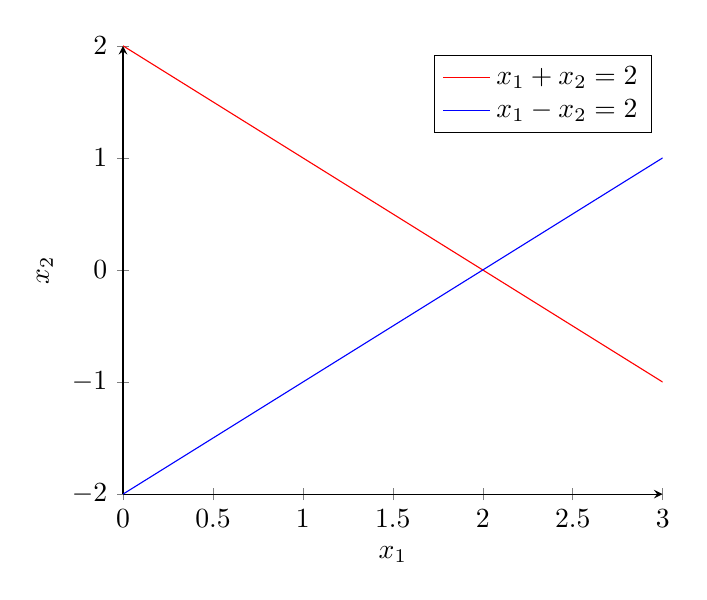
\begin{tikzpicture}
\begin{axis}[
    axis lines = left,
    xlabel = $x_1$,
    ylabel = {$x_2$},
]
%Below the red parabola is defined
\addplot [
    domain=0:3, 
    samples=100, 
    color=red,
]
{2-x};
\addlegendentry{$x_1+x_2=2$}
%Here the blue parabloa is defined
\addplot [
    domain=0:3, 
    samples=100, 
    color=blue,
    ]
    {x-2};
\addlegendentry{$x_1-x_2=2$}
\end{axis}
\end{tikzpicture}
\end{center}
\paragraph{Case2: no solution} If two lines are parallel, then there is no solution.
\begin{center}
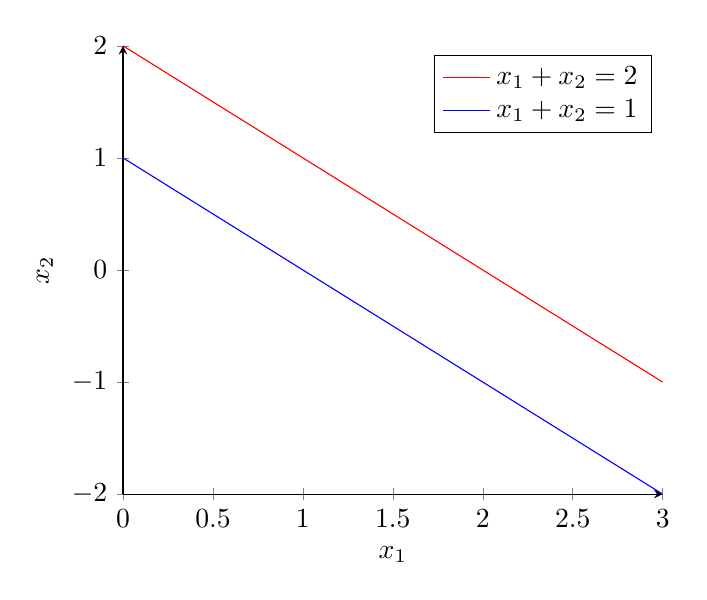
\begin{tikzpicture}
\begin{axis}[
    axis lines = left,
    xlabel = $x_1$,
    ylabel = {$x_2$},
]
%Below the red parabola is defined
\addplot [
    domain=0:3, 
    samples=100, 
    color=red,
]
{2-x};
\addlegendentry{$x_1+x_2=2$}
%Here the blue parabloa is defined
\addplot [
    domain=0:3, 
    samples=100, 
    color=blue,
    ]
    {1-x};
\addlegendentry{$x_1+x_2=1$}
\end{axis}
\end{tikzpicture}
\end{center}
\paragraph{Case 3: infinite number of solutions} If both equations represent the same line, then there are infinite number of solutions.
\begin{center}
\begin{tikzpicture}
\begin{axis}[
    axis lines = left,
    xlabel = $x_1$,
    ylabel = {$x_2$},
]
%Below the red parabola is defined
\addplot [
    domain=0:3, 
    samples=100, 
    color=red,
]
{2-x};
\addlegendentry{$x_1+x_2=2$}
%Here the blue parabloa is defined
\addplot [
    domain=0:3, 
    samples=100, 
    color=blue,
    ]
    {2-x};
\addlegendentry{$-x_1-x_2=-2$}
 
\end{axis}
\end{tikzpicture}
\end{center}
\subsubsection{How to solve $3 \times 3$ Systems?}

\begin{example} \qquad
\\
Let's recall how to solve a $3 \times 3$ system equations as below:

\[
\left \{	\begin{gathered}
2x_1 + x_2 +x_3=5 	\\
4x_1 + (-6)x_2 = -2 \\
-2x_2+7x_2+2x_3 = 9
\end{gathered}	\right.
\]
We can simplify the equation system above into the \emph{Augmented matrix} form:
\[
\left \{	\begin{gathered}
2x_1 + x_2 +x_3=5 	\\
4x_1 + (-6)x_2 = -2 \\
-2x_2+7x_2+2x_3 = 9
\end{gathered}	\right.
\qquad \implies \qquad
\left[
\begin{array}{@{}ccc|c@{}}
2 & 1 & 1 & 5\\
4 & -6 & 0 & -2\\
-2 & 7 & 2 & 9
\end{array}
\right]
\]
%
\[
\xLongrightarrow[\text{Add row 1 to row 3}]{\text{Add $(-2)\times$ row 1 to row 2}}{\quad\quad}
\left[
\begin{array}{@{}ccc|c@{}}
2 & 1 & 1 & 5\\
0 & -8 & -2 & -12\\
0 & 8 & 3 & 14
\end{array}
\right]
\]
\[\xLongrightarrow{\text{Add row 2 to row 3}}{\quad\quad}
\left[
\begin{array}{@{}ccc|c@{}}
2 & 1 & 1 & 5\\
0 & -8 & -2 & -12\\
0 & 0 & 1 & 2
\end{array}
\right]\]
This augmented matrix is the \emph{strictly triangular system}, and it's trial to get the final solution:
\[\implies
\begin{pmatrix}
x_1\\x_2\\x_3
\end{pmatrix}=
\begin{pmatrix}
1\\1\\2
\end{pmatrix}\]
\end{example}

Here we give the definition for strictly triangular system:
\begin{definition}[strictly triangular system]
For the augmented matrix
\[
\left[
\begin{array}{@{}cccc|c@{}}
a_{11} & a_{12} & \dots & a_{1n} &  b_1 \\
a_{21} & a_{22} & \dots & a_{2n} &  b_2 \\
\vdots    & \vdots    & \ddots & \vdots    & \vdots \\
a_{m1} & a_{m2} & \cdots & a_{mn} &   b_n
\end{array}
\right],
\]
if in the $k$th row, the first $(k-1)$th column entries are \textit{all zero} and the $k$th column entries is nonzero, we say the augmented matrix(or corresponding system equation) is of \emph{strictly triangular form}. This kind of matrix(or corresponding system equation) is called \emph{strictly triangular system}.
$(k = 1, . . . , m).$
\end{definition}

\subsubsection{How to solve $n \times n$ System?}
We try to reduce an $n \times n$ System to strictly triangular form. Let's take a special example:
\begin{example}
Given an $n \times n$ System of the form:
\begin{equation}\left[
\begin{array}{@{}cccc|c@{}}
a_{11} & a_{12} & \dots & a_{1n} &  b_1 \\
a_{21} & a_{22} & \dots & a_{2n} &  b_2 \\
\vdots    & \vdots    & \ddots & \vdots    & \vdots \\
a_{n1} & a_{n2} & \cdots & a_{nn} &   b_n
\end{array}\right]\label{eq:n*n_matrix}\end{equation}
Assuming the \emph{diagonal entries} are always \textit{nonzero} during our operation. 
Add row 1 that multiplied by a constant to other $n-1$ row to ensure the first entry of other $n-1$ rows are all \textit{zero}:
\begin{equation}
\implies 
\left[
\begin{array}{@{}cccc|c@{}}
a_{11} & a_{12} & \dots & a_{1n} &  b_1 \\
0 & \x & \dots & \x &  \x \\
\vdots    & \vdots    & \ddots & \vdots    & \vdots \\
0 & \x & \cdots & \x &   \x
\end{array}
\right] \label{eq:n*n_matrix_version1}\end{equation}


Then we proceed this way $n-1$times to obtain:
\begin{equation}
  \left[
    \begin{array}{@{}ccccc|c@{}}
    \x    & \x       & \x    & \x    & \x & \x\\ \cline{1-1}
    \bord & \x       & \x    & \x    & \x & \x\\ \cline{2-2}
          & \bord    & \x    & \x    & \x & \vdots \\ \cline{3-3}
          & \bigzero & \bord & \x    & \x & \vdots \\ \cline{4-4}
          &          &       & \bord & \x & \x \\ \cline{5-5}
  \end{array}\right]\label{eq:n*n_matrix_version2}
\end{equation}

This matrix is the \emph{Row-echelon form}.
And we do the back substitution again to obtain:
\begin{equation}
  \left[
    \begin{array}{@{}ccccc|c@{}}
    \x    &        &     &     &  & \x\\ \cline{1-1}
    \bord & \x       &     &     & \bigzero & \x\\ \cline{2-2}
          & \bord    & \x    &     &  & \vdots \\ \cline{3-3}
          & \bigzero & \bord & \x    &  & \vdots \\ \cline{4-4}
          &          &       & \bord & \x & \x \\ \cline{5-5}
  \end{array}\right]\label{eq:n*n_matrix_version3}
\end{equation}
This matrix is the \emph{Reduced Row-Echelon Form}.
Finally by multiplying every row by a nonzero constant to ensure its \emph{diagnoal entries} are all $1$:
\begin{equation}
  \left[
    \begin{array}{@{}ccccc|c@{}}
    1    &        &     &     &  & \x\\ \cline{1-1}
    \bord & 1       &     &     & \bigzero & \x\\ \cline{2-2}
          & \bord    & \ddots    &     &  & \vdots \\ \cline{3-3}
          & \bigzero & \bord & 1    &  & \vdots \\ \cline{4-4}
          &          &       & \bord & 1 & \x \\ \cline{5-5}
  \end{array}\right]\label{eq:n*n_matrix_version4}
\end{equation}
\end{example}

Then let's analysis the complexity of solving such a $n\times n$ system.
\subsection{Complexity Analysis}
\subsubsection{Step1: Reduction from matrix (\ref{eq:n*n_matrix}) to matrix (\ref{eq:n*n_matrix_version1})}
\begin{proposition}
The time complexity for Augmented matrix reduction using back-substitution algorithm is $\mathcal{O}(n^3)$.
\end{proposition}

\begin{proof}
The estimation for the time complexity requires us to estimate how many steps of \emph{multiplication} we need. (The time for addition is so small that can be ignored).
\begin{itemize}
\item
Reducing matrix (\ref{eq:n*n_matrix}) to matrix (\ref{eq:n*n_matrix_version1}) we need to do $n(n-1)$times multiplications.

This is because for each row (except first row) we have known the first entry is zero, while the remaining $(n-1)$ entries in each row should be computed by multiplying first row's entries and then add it to the row.
\item
Then it suffices to deal with the inner $(n-1)\times (n-1)$ matrix, which requires the $(n-1)\times (n-2)$ times multiplication.
\item
The back substitution for matrix (\ref{eq:n*n_matrix}) requires $n$ times reduction.
\end{itemize}
Hence the total multiplication times for back substitution for matrix (\ref{eq:n*n_matrix}) is
\begin{equation*}
\begin{split}
\sum_{i=1}^n i(i-1)
	&= \sum_{i=1}^n (i^2-i)  \\
 		&=\sum_{i=1}^n i^2 - \sum_{i=1}^n i \\
		&=\frac{n(n+1)(2n+1)}{6} - \frac{n(n+1)}{2} \\
		&=\frac{n^3-2n}{3} \sim \frac{n^3}{3} =O(n^3)
\end{split}
\end{equation*}
\end{proof}
But we can always develop more advanced algorithm that have smaller time complexity.

\subsubsection{Step2: Reduction from triangular system to diagonal system}

In order to reducing matrix (\ref{eq:n*n_matrix_version2}) to matrix (\ref{eq:n*n_matrix_version3}) we need to do back-substitution again. The matrix (\ref{eq:n*n_matrix_version3}) is diagonal system. Obviously, for this process the total multiplication times is given by
\[
1+2+\cdots+n-1 = \frac{n(n-1)}{2} \sim O(n^2)
\]
\subsubsection{Step3: Get final solution}

In the final step, we want to reduce matrix (\ref{eq:n*n_matrix_version3}) to matrix (\ref{eq:n*n_matrix_version4}), the only thing we need to do is to do one multiplication for each row to let the diagonal entries be $1$. Hence the total multiplication times for this process is given by
\[
\underbrace{1+1+\dots+1}_{\text{totally $n$ terms}} = O(n)
\]
\subsection{Brief Summary}
The reduction of $n\times n$ matrix requires three kinds of Row operations:
\begin{itemize}
\item \emph{Addition and Multiplication}.

Add to a row by a constant multiple of another row.

\item \emph{Multiplication}

Multiply a row by a nonzero constant.
\item \emph{Interchange}

Interchange two rows
\end{itemize}


\begin{enumerate}
\item
agds
\end{enumerate}•